\documentclass{article}
\usepackage[utf8]{inputenc}
\usepackage[a4paper, margin=1in]{geometry}
\usepackage{fancyhdr}
\usepackage{titlesec}
\usepackage[backend=bibtex,style=ieee]{biblatex}
\usepackage{hyperref}
\usepackage{graphicx}
\usepackage{algorithm}
\usepackage{algpseudocode}
\usepackage{float}
\usepackage{multicol}
\usepackage{url}

\addbibresource{references.bib}

\title{Kernel Image Processing}
\author{Luka Uršič \\ 89221145 \\ UP Famnit \\ E-mail: 89221145@student.upr.si}
\date{\today}

\pagestyle{fancy}
\fancyhf{}
\rhead{\today}
\lhead{Kernel Image Processing}
\rfoot{Page \thepage}
\titleformat{\section}
{\normalfont\Large\bfseries}{\thesection}{1em}{}

\begin{document}

\maketitle
\thispagestyle{empty}

\begin{abstract}
    In this paper, I present how to use kernel image processing to modify an image. I explain how kernel image processing works, how I implemented it, and the time results I obtained from running it sequentially, in parallel, and with distributed computing. I compare the results and conclude which method is the best for this specific task.
\end{abstract}

\begin{multicols}{2}

    \section{Introduction}
    An image kernel is a number matrix used to apply effects like the ones you might find in popular photo manipulation software, such as blurring, sharpening, outlining, or embossing. They're also used in machine learning for 'feature extraction', a technique for determining the most important portions of an image. In this context, the process is referred to more generally as "convolution".
    \cite{setosa}

    \section{Convolution}

    \subsection{Definition}

    Here is the mathematical definition of the convolution of original image $f(x, y)$, kernel $\omega$, and resulting image $g(x, y)$:

    \begin{equation}
        g(x, y) = \omega * f(x, y) = \sum_{i=-a}^{a} \sum_{j=-b}^{b} \omega(i, j) f(x-i, y-j)
    \end{equation}
    \cite{wikipedia}

    \subsection{Explanation}

    To perform a convolution, the program uses a kernel that is applied to each pixel in the image. This kernel works by interacting with the pixel and its surrounding neighbors. The value of the new pixel is calculated through a process where the pixels are multiplied by the corresponding values in the kernel and then summed up. The result is a pixel on a new image. The kernel is then moved to the next pixel. See figure \ref{fig:kernel} for a visual representation.

    \begin{figure}[H]
        \centering
        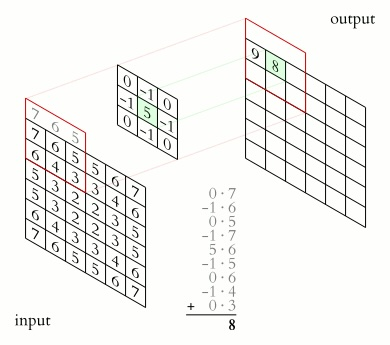
\includegraphics[width=\linewidth]{img/kernel.jpg}
        \caption{Convolution of an image with a kernel, illustrating how the output pixel value is calculated}
        \label{fig:kernel}
    \end{figure}

    By systematically applying the kernel across the entire image, the program can achieve the desired transformation or effect, that can be used in image manipulation programs or machine learning algorithms.

    Processing an image sequentially, pixel by pixel, is inefficient, especially for large images and can be time-consuming. To overcome this, parallel computing offers a compelling solution, by partitioning the image into smaller, independent sub-images. These sections can be processed concurrently across multiple threads. Data used by different threads is not depending on one another, which makes it a trivially parallel problem. This approach can drastically accelerate image processing tasks compared to sequential methods.

    \section{Implementation}
    I implemented Kernel Image Processing in Java and used the Swing and AWT libraries to display the images.

    I created a class called ImageProcessor that contains the methods applyKernelToPixel, applyKernelSequential, and applyKernelParallel. The applyKernelToPixel method applies the kernel to a single pixel, the applyKernelSequential method applies the kernel to the image sequentially, and the applyKernelParallel method applies the kernel to the image in parallel.

    You can see the pseudocode for the class ImageProcessor in the following algorithm.

    \begin{algorithm}[H]
        \caption{Pseudocode for ImageProcessor.java}
        \raggedright
        \begin{algorithmic}[1]
            \State \textbf{Class} ImageProcessor
            \State
            \State \textbf{Function} applyKernelToPixel(origImg, kernel, newImg, x, y)
            \State Initialize r, g, b to 0
            \For{each value in kernel}
            \State Add (origImg pixel \(*\) kernel value)
            \EndFor
            \State Clamp r, g, b to [0, 255]
            \State Set newImg at (x, y) to (r, g, b) to r, g, b
            \State \textbf{End Function}
            \State
            \State \textbf{Function} applyKernelSequential(origImg, kernel)
            \State Initialize newImg
            \For{each pixel (x, y) in origImg}
            \State Call applyKernelToPixel(origImg, kernel, newImg, x, y)
            \EndFor
            \State \textbf{Return} newImg
            \State \textbf{End Function}
            \State
            \State \textbf{Function} applyKernelParallel(origImg, kernel)
            \State Initialize newImg
            \State Use ForkJoinPool to process pixels in parallel
            \State \textbf{Return} newImg
            \State \textbf{End Function}
            \State
            \State \textbf{End Class}
        \end{algorithmic}
    \end{algorithm}

    \subsection{Sequential implementation}

    The applyKernelSequential method processes each pixel in the image one by one, row by row. This method is simple and easy to implement, but it can be slow for large images.

    \subsection{Parallel implementation}

    The applyKernelParallel method applies the kernel to the image in parallel using a ForkJoinPool that has threads corresponding to the number of computer processors. Then pixels are submitted to the pool and automatically asigned to any thread. I used ForkJoinPool because of these advantages:

    \begin{itemize}
        \item \textbf{Work-Stealing Algorithm}: It  distributes tasks to idle threads for balanced workload.
        \item \textbf{Lower Overhead}: It reuses threads instead of creating new ones, reducing overhead.
        \item \textbf{Built-in Java Framework}: It is part of the Java standard library, making it easy to use.
    \end{itemize}

    \newblock

    Here is the code for the parallel processing:

    \begin{figure}[H]
        \centering
        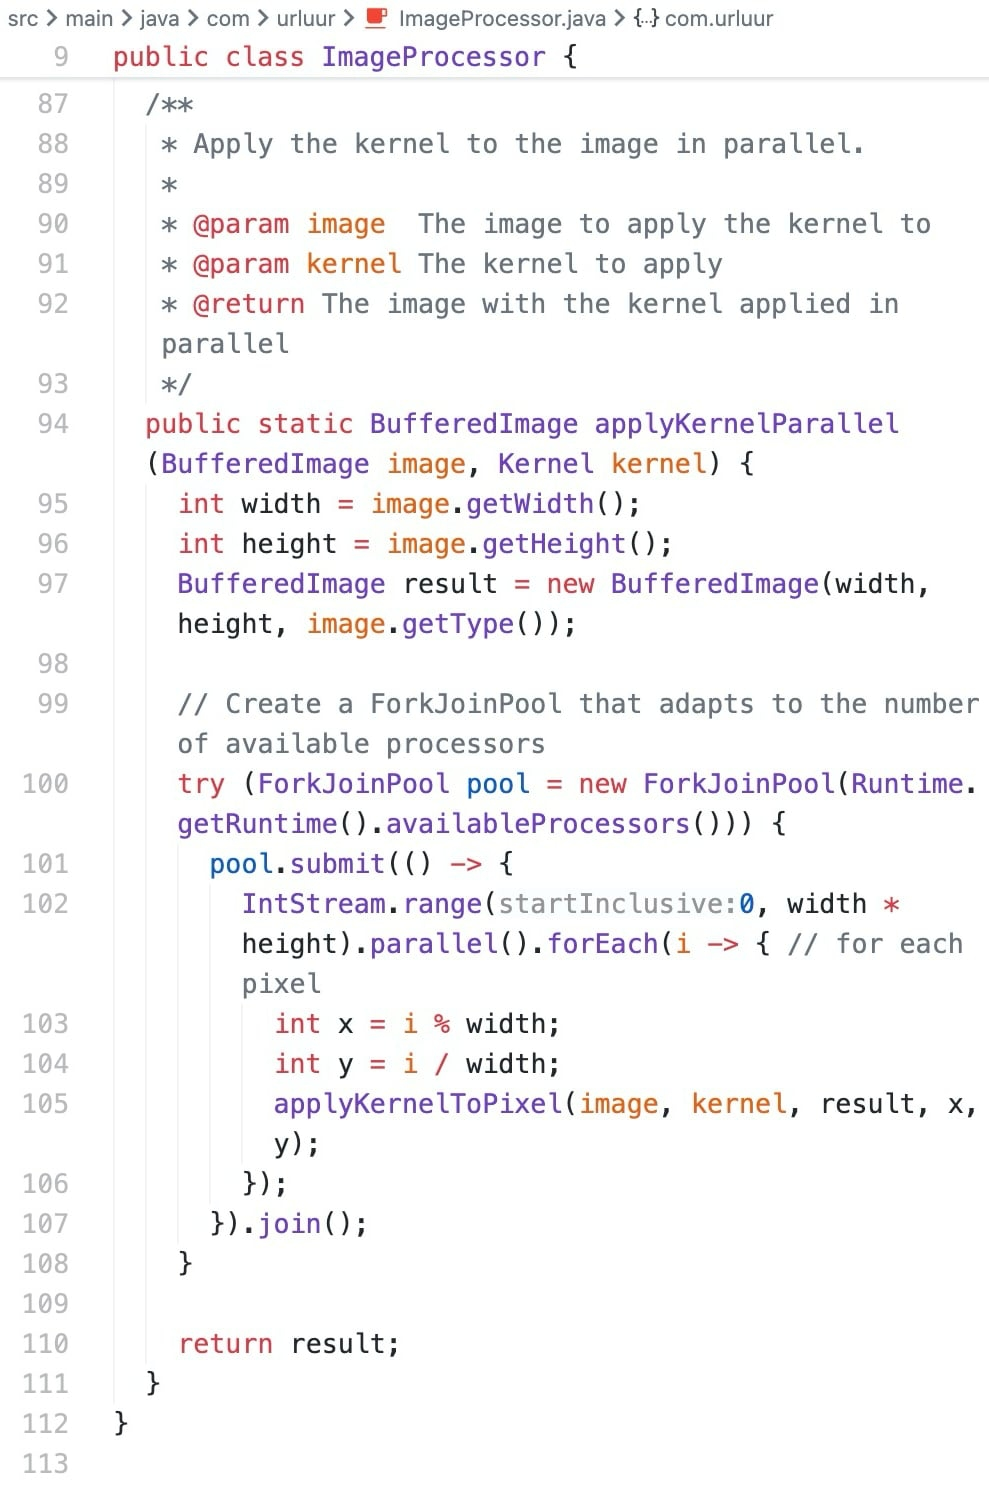
\includegraphics[width=\linewidth]{img/parallel.jpg}
        \caption{Code for parallel processing that submits each pixel to the ForkJoinPool}
        \label{fig:parallelcode}
    \end{figure}

    Later I implemented parallel mode that splits the image into smaller chunks and processes them in parallel. This way, the processing time is further reduced due to less overhead. Its implementation is a bit more complicated, but both are similar. I decided to keep both implementations, so the user can choose which mode to use.

    \subsection{Distributed implementation}

    For distributed computing I used MPI (Message Passing Interface) in MPJ Express. I split the image into smaller parts and sent them to other machines for processing. The results were then sent back to the main machine and combined to form the final image.

    \subsubsection{Key Methods}

    \begin{itemize}
        \item \texttt{masterDistributed}: This method sends the image and kernel to the workers, then processes one chunk of the image. It then receives the results from the workers and combines them to form the final image.

        \item \texttt{workerDistributed}: This method receives the chunk of an image and kernel from the master, processes the chunk, and sends the results back to the master.

        \item \texttt{applyKernelDistributed}: This method is used by master and workers to process a chunk of the image using the kernel.

    \end{itemize}

    \subsubsection{Performance Considerations}

    While distributed computing can theoretically provide significant performance improvements, the actual performance gains depend on several factors:
    \begin{itemize}
        \item \textbf{Network Latency}: The time taken to send and receive chunks over the network can impact performance.
        \item \textbf{Data Transfer Overhead}: Large images have significant overhead because of their size.
        \item \textbf{Synchronization}: Ensuring that all chunks are combined correctly can introduce additional delays.
    \end{itemize}

    \section{Testing environment}
    I tested the program on my laptop computer with the following specifications:

    \begin{itemize}
        \item \textbf{Processor}: Apple M1 chip
        \item \textbf{RAM}: 8 GB unified memory
        \item \textbf{Operating System}: macOS Sonoma
        \item \textbf{Java Version}: OpenJDK 22
        \item \textbf{MPI Version}: MPJ Express 0.44
    \end{itemize}

    \section{Results}

    I tried running the program in sequential mode and in parallel mode with the demo picture of coffee of three different sizes. Results in sequential mode were following the number of pixels in the image. The results in parallel mode were much faster than in sequential mode.

    The difference was significant. It noted speedups of nearly up to 4x. I assume that the speedup number is connected to the number of processor cores. Such speedup was present when processing small and large images.

    \begin{figure}[H]
        \centering
        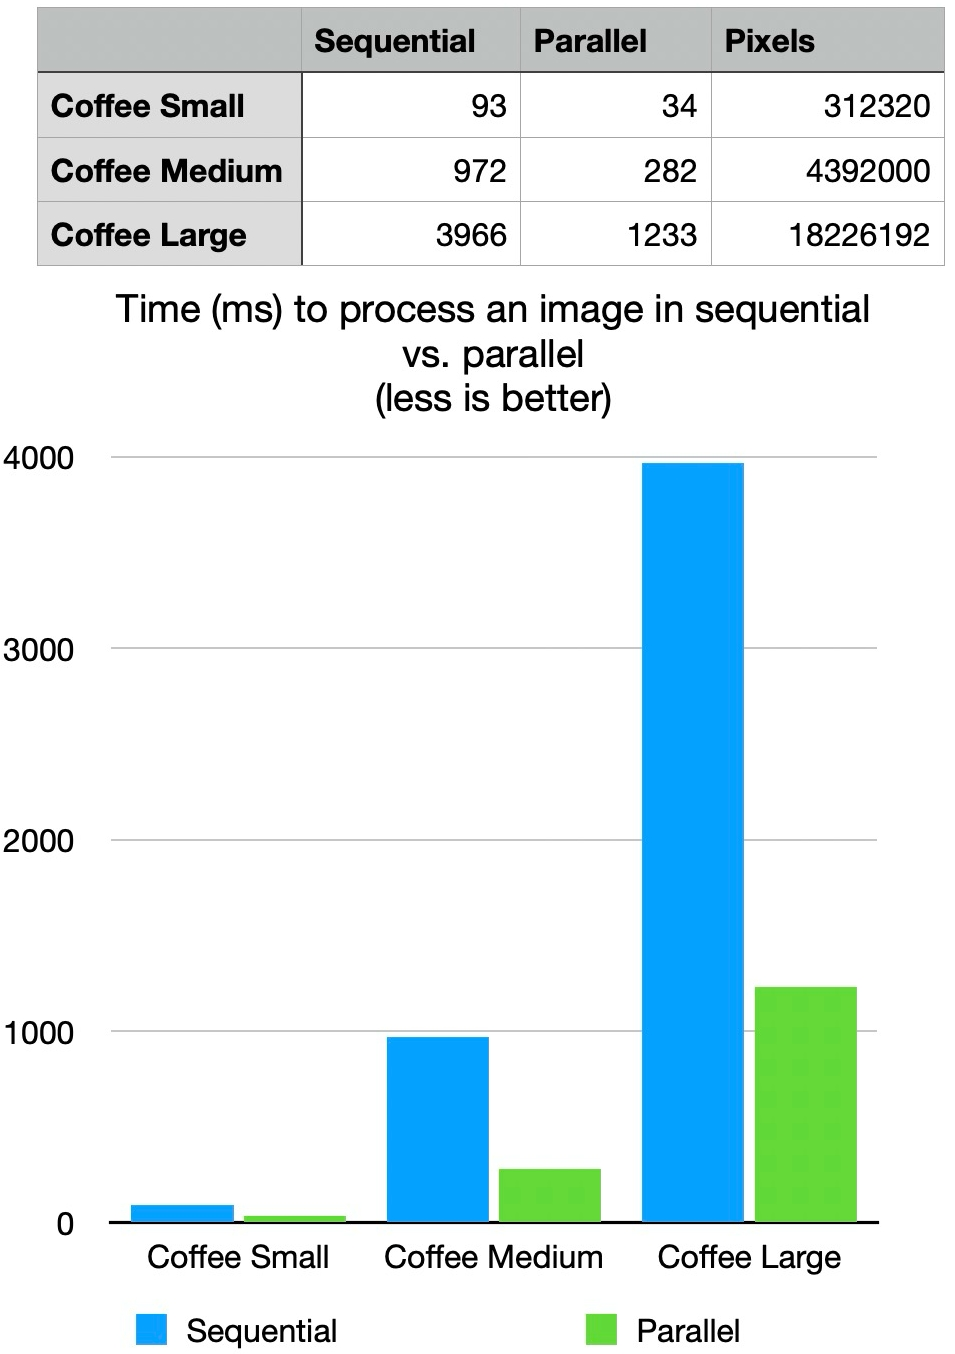
\includegraphics[width=\linewidth]{img/parallel_speedup.jpg}
        \caption{Initial speedup comparison between sequential and parallel processing}
        \label{fig:speedup}
    \end{figure}

    I was satisfied with the results of the parallel processing, compared to the very slow sequential approach. This proves the problem is really trivially parallel problem.

    However, operating system, processor temperature and other programs running in the background can affect the results.

    \pagebreak

    \subsection{Average measurements}
    Because of the slightly inconsistent measurements, I decided to run the it 10 times and take the average. The results were consistent, and the speedup was still present. The average speedup was around 3.5x.

    In the same way, I measured the average times of all implemented modes. The data is shown in the following table.

    \begin{figure}[H]
        \centering
        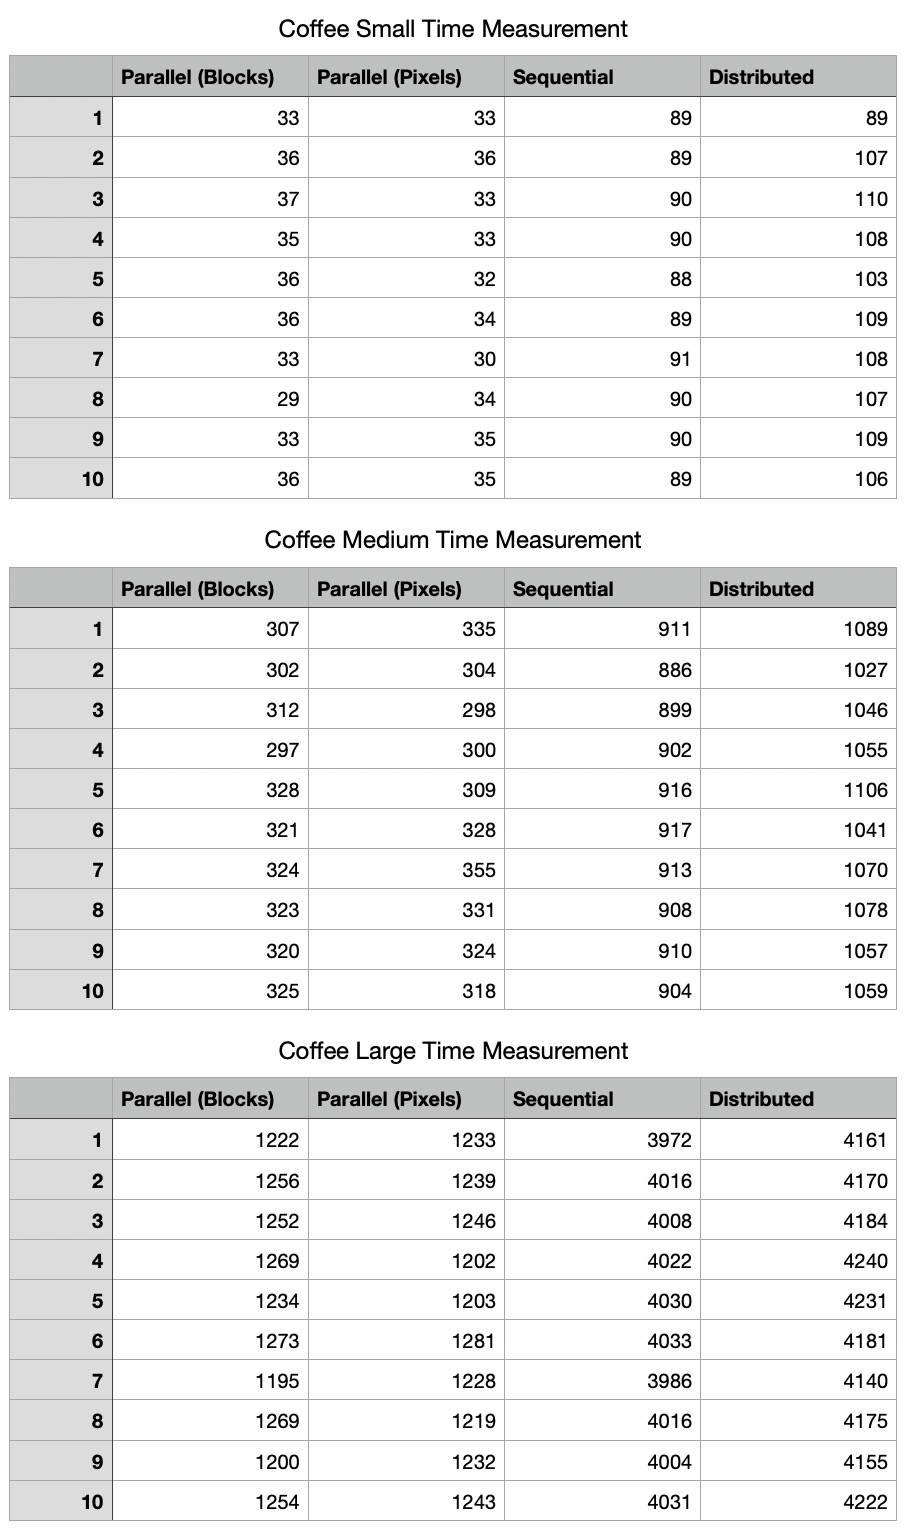
\includegraphics[width=\linewidth]{img/measurements.jpg}
        \caption{Measurements of processing times}
        \label{fig:modes}
    \end{figure}

    I noticed that the time it took to process the image in distributed mode was slower than in sequential. This was surprising to me, as I expected distributed computing to be much faster, evem faster than parallel, but it turns out it was the slowest.

    The distributed mode was actually very close to sequential mode, so I compared the two in the graph. Both parallel versios were way ahead of the other two modes, but the tested images were not large enough to see any significant difference between the two parallel modes.

    \begin{figure}[H]
        \centering
        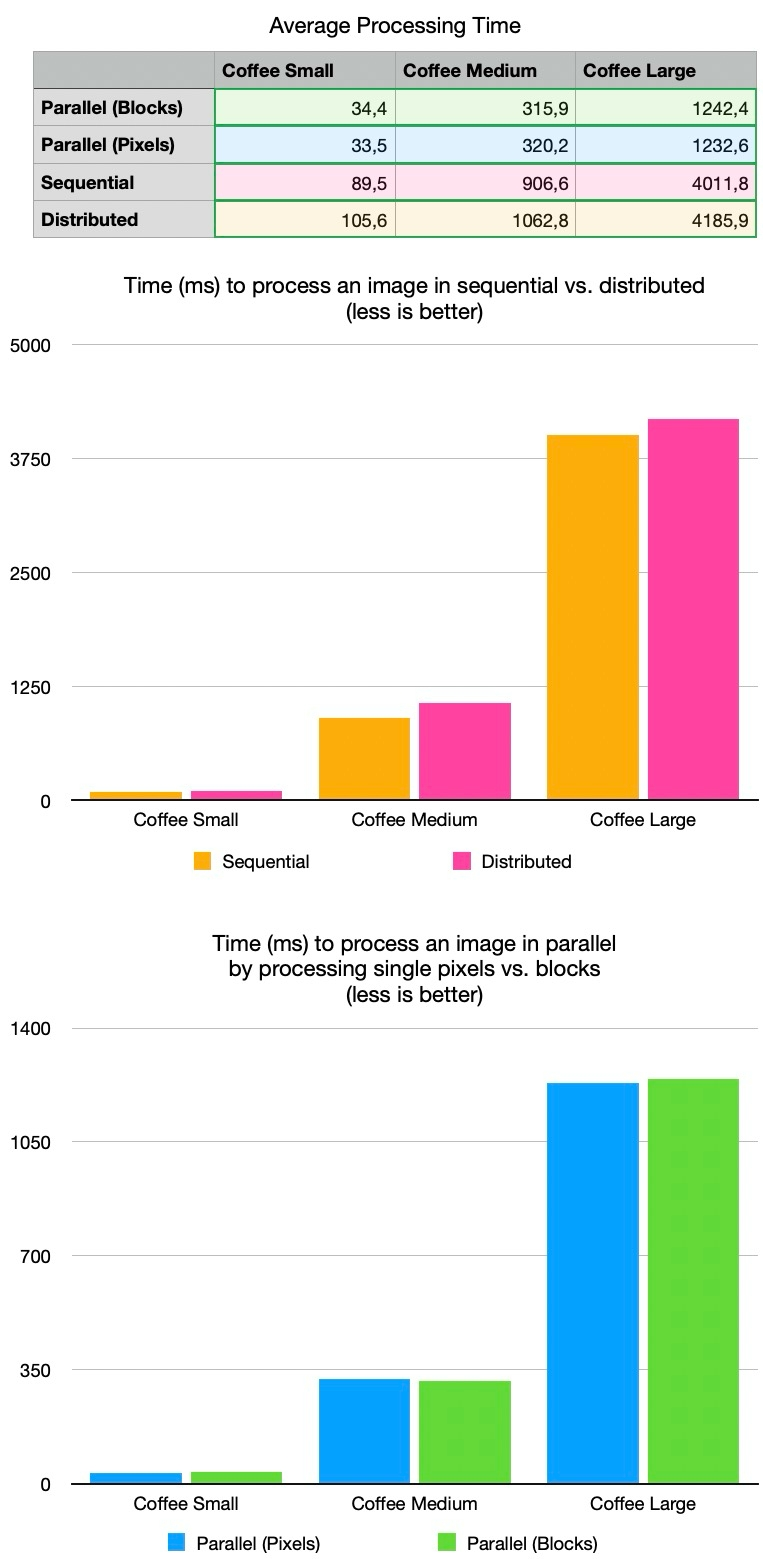
\includegraphics[width=\linewidth]{img/average_detailed.jpg}
        \caption{All Average Measurements}
        \label{fig:distributed}
    \end{figure}

    The reason for distributed mode not reaching my expectations is that the overhead of sending the chunks of an image was too high.

    \section{Conclusion}

    The results of my experiments show that parallel computing using a ForkJoinPool provides significant speedup compared to sequential processing. The speedup was observed for both small and large images, indicating that parallel processing is beneficial regardless of image size.

    However, the distributed computing approach did not yield better performance compared to parallel computing. The overhead of sending the image to other machines outweighed the potential benefits of distributed processing.

\end{multicols}

\printbibliography[heading=bibintoc, title={References}]

% // TODO: Dodaj reference na kakšen članek o konvoluciji oziroma parallel implementaciji kernel image processing

\end{document}